%xelatex -shell-escape -output-directory=bin ergasia.tex
\documentclass{assignment}

\university{Πανεπιστήμιο Πειραιώς}{Πα.Πει.}
\school{Τμήμα Πληροφορικής}{Π.Μ.Σ. "Πληροφορική"}
\department{Πρόγραμμα Μεταπτυχιακών Σπουδών «Πληροφορική»}{}
%\cover{images/cover.jpg}{http://www.cyberciti.biz/faq/grub-boot-into-single-user-mode/}

\title{Τεχνολογίες Διαδικτύου \\ 4η Εργασία}
%\projectlevel{Εργαστήριο Λειτουργικά Συστήματα}
%\lesson{Λειτουργικά Συστήματα}{1}
\date{Αθήνα, 2014}

\author{Αναγνωστόπουλος Βασίλης - Θάνος, Κατσής Γεώργιος}
%\register{ΜΠΠΛ13002}{1}

%\exercauthor{Αναγνωστόπουλος Βασίλης - Θάνος}{06107083}{9}

%\advisor{Τσακίρη Μαρία, Αναπληρώτρια Καθηγήτρια Ε.Μ.Π.}

\begin{document}

\maketitle
% Να σκεφτώ τί αλλαγές θέλω να κάνω με τις αριθμήσεις και άμα θέλω να κάνω.
% Να σκεφτώ να τις ενσωματώσω και στο assignment.cls

\setcounter{page}{1} 
\pagenumbering{roman}

\pagestyle{plain}
\tableofcontents
\newpage


%\pagestyle{headings}
\pagestyle{fancy}
\setcounter{page}{1} 
\pagenumbering{arabic}

\begin{Assignment}%[Ερώτημα]
\AssignmentTitle{ % 
Δημιουργήστε μία ιστοσελίδα παραγγελίας προϊόντων ή υπηρεσιών.

Η ιστοσελίδα θα πρέπει να περιλαμβάνει μία φόρμα HTML, στην οποία ο χρήστης
θα μπορεί να επιλέγει τα προϊόντα ή τις υπηρεσίες που επιθυμεί, να εισάγει τα στοιχεία του , να προσδιορίζει τον τρόπο πληρωμής και εάν χρειάζεται
να δίνει τον αριθμό της πιστωτικής του κάρτας.

Η φόρμα θα πρέπει, επίσης, να περιέχει δύο πλήκτρα με τίτλους “Παραγγελία” και “Ακύρωση”. Όταν ο χρήστης επιλέγει το πλήκτρο “Ακύρωση” θα επανεμφανίζονται οι προκαθορισμένες τιμές των πεδίων της φόρμας, ενώ όταν επιλέγει το πλήκτρο “Παραγγελία” θα εκτελείται ένα σενάριο JavaScript.

Το σενάριο θα ελέγχει εάν έχουν επιλεγεί κάποια προϊόν τα ή υπηρεσίες, εάν έχουν συμπληρωθεί σωστά τα στοιχεία που αφορούν το χρήστη, εάν έχει προσδιοριστεί τρόπος πληρωμής και, σε περίπτωση που χρειάζεται, εάν έχει δοθεί αριθμός πιστωτικής κάρτας με 16 ψηφία. Σε περίπτωση λάθους, θα εμφανίζει κατάλληλο μήνυμα. Διαφορετικά, θα υπολογίζει τη συνολική τιμή της
παραγγελίας και θα την εμφανίζει σε ένα πεδίο κειμένου της ίδιας σελίδας.

Παρατήρηση:
Η ιστοσελίδα θα πρέπει να μορφοποιείται με κανόνες CSS, που περιλαμβάνονται σε ένα εξωτερικό αρχείο. 
}

Ο κώδικας που υλοποιεί την σελίδα φαίνεται παρακάτω.

Για την συνάρτηση που ελέγχει αν είναι έγκυρη η παραγγελία έχουν γίνει οι παρακάτω παραδοχές:
\begin{itemize}
\item Το μήκος του ονόματος και του επιθέτου πρέπει να είναι μεγαλύτερο του μηδενός
\item Το μήκος του τηλεφώνου πρέπει είναι δέκα χαρακτήρες
\item Το μήκος της πιστωτικής κάρτας πρέπει να είναι 16 χαρακτήρες
\end{itemize}

\inputminted[linenos,tabsize=2]{html}{../../index.html}
\captionof{listing}{Ο κώδικας της σελίδας \label{html_code}}

\inputminted[linenos,tabsize=2]{css}{../../theme.css}
\captionof{listing}{Ο κώδικας css της σελίδας \label{css_code}}

\inputminted[linenos,tabsize=2]{js}{../../javascript.js}
\captionof{listing}{Ο κώδικας javascript της σελίδας \label{javascript_code}}

Ακόμα ο κώδικας της βρίσκεται στο \url{https://github.com/giokats/Texnologies_Diadiktiou}
\end{Assignment}

Τέλος ο κώδικας της σελίδας ελέγχθηκε χρησιμοποιώντας το \url{http://validator.w3.org} (εικόνα 
\ref{fig:date})

\begin{figure}
\begin{center}
\resizebox*{!}{8.5cm}{
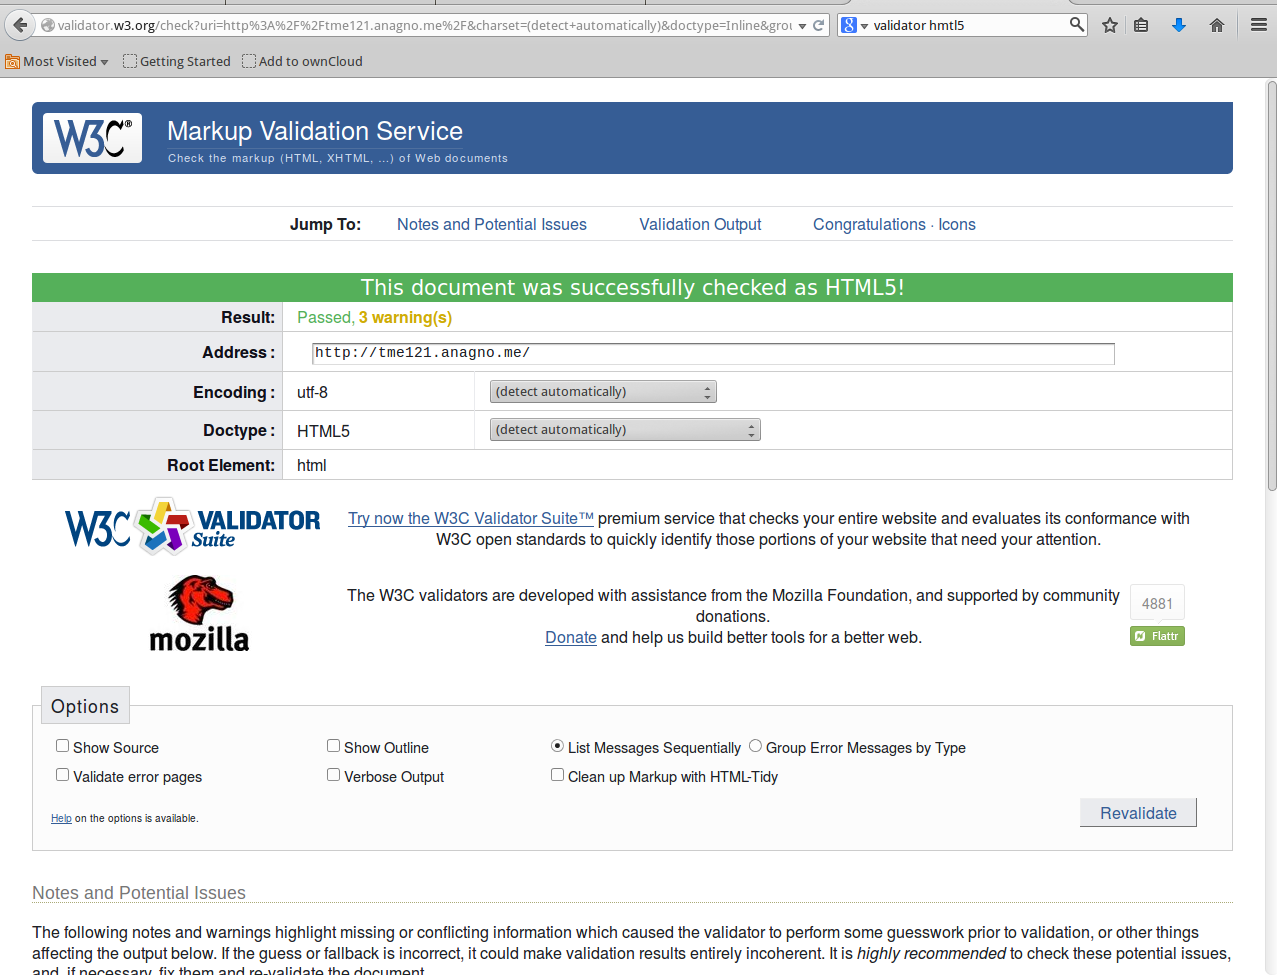
\includegraphics{images/validator.png}}
\caption{Screenshot από το \url{http://validator.w3.org} }
\label{fig:date}
\end{center}
\end{figure}

\begin{figure}
\begin{center}
\resizebox*{!}{8.5cm}{
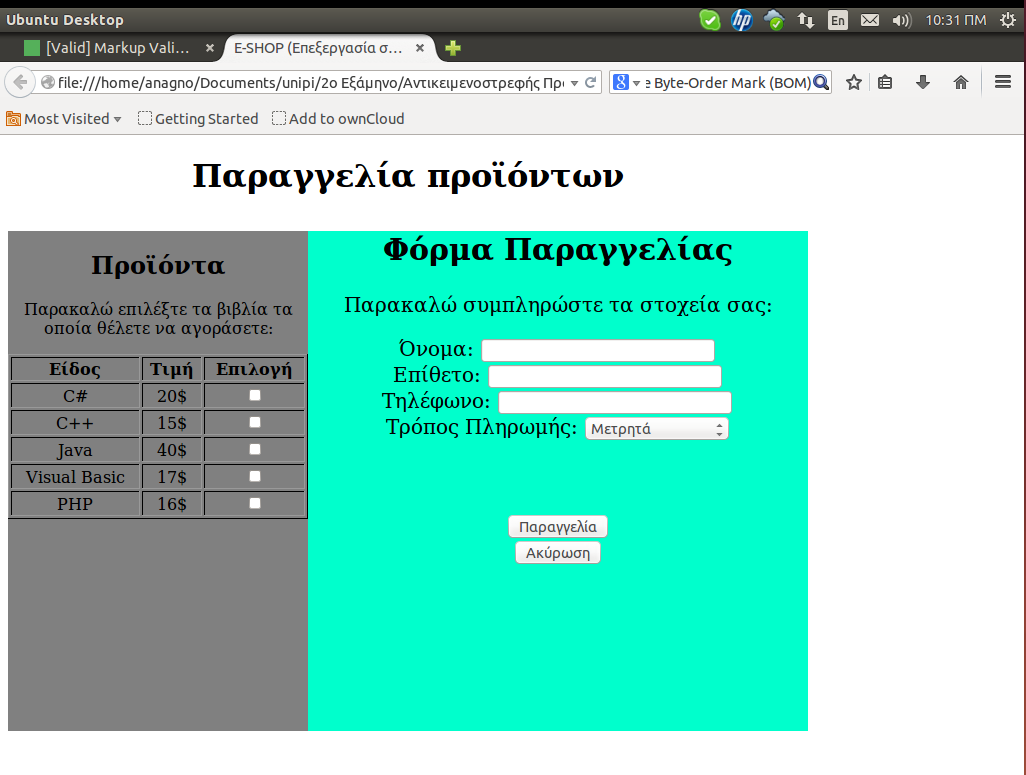
\includegraphics{images/site.png}}
\caption{Screenshot από την ιστοσελίδα χρησιμοποιώντας τον \en{firefox} }
\label{fig:site}
\end{center}
\end{figure}


%\phantomsection \label{Βιβλιογραφία}
%\addcontentsline{toc}{section}{Βιβλιογραφία}
%\mtcaddchapter[Βιβλιογραφία] % Λόγω του minitoc
%\bibliographystyle{plain}
%\bibliography{references}

\newpage

\end{document}

